\chapter{Background}
\label{ch:background}

This chapter discusses the key concepts that are required to understand the Thesis work.

\section{Static Analysis}

In the last few years, we see the enormous increase in the usage of Software. We see the presence of Software everywhere in the walk of our life with the Internet of Things, for example. As the usage increases, quality is stressed as to be more secure and it does not break. Earlier, Software developers used to do manual auditing of the code but sooner they realised it is time-consuming and so planned to automate the process. Therefore, different testing mechanisms evolved like black-box testing, white-box testing etc. \\ \\

Static Analysis falls under the category White-box testing. It tests the Software without executing the code and therefore the name means it. On the other side, there are tools testing with a mechanism by executing the code which is called Dynamic testing. Static Analysis is also called as Source Code Analysis. There are different techniques followed for analysing Source Code. One example as Data Flow Analysis, it tests the source code by dividing into basic blocks \cite{Woegerer}. Here is an example; a php program as seen in figure is divided into blocks and each block is considered as one node as seen in figure \ref{fig:php}. Thereafter, a path is formed by connecting the nodes along the control flow as seen in figure \ref{fig:cfg}. \\ \\

\begin{figure}[H]
	\centering
	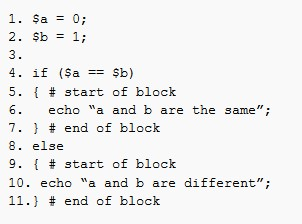
\includegraphics[scale=0.5]{figures/PHP-code}
	\caption{PHP Code with Basic Blocks.}
	\label{fig:php}
\end{figure}

\begin{figure}[H]
	\centering
	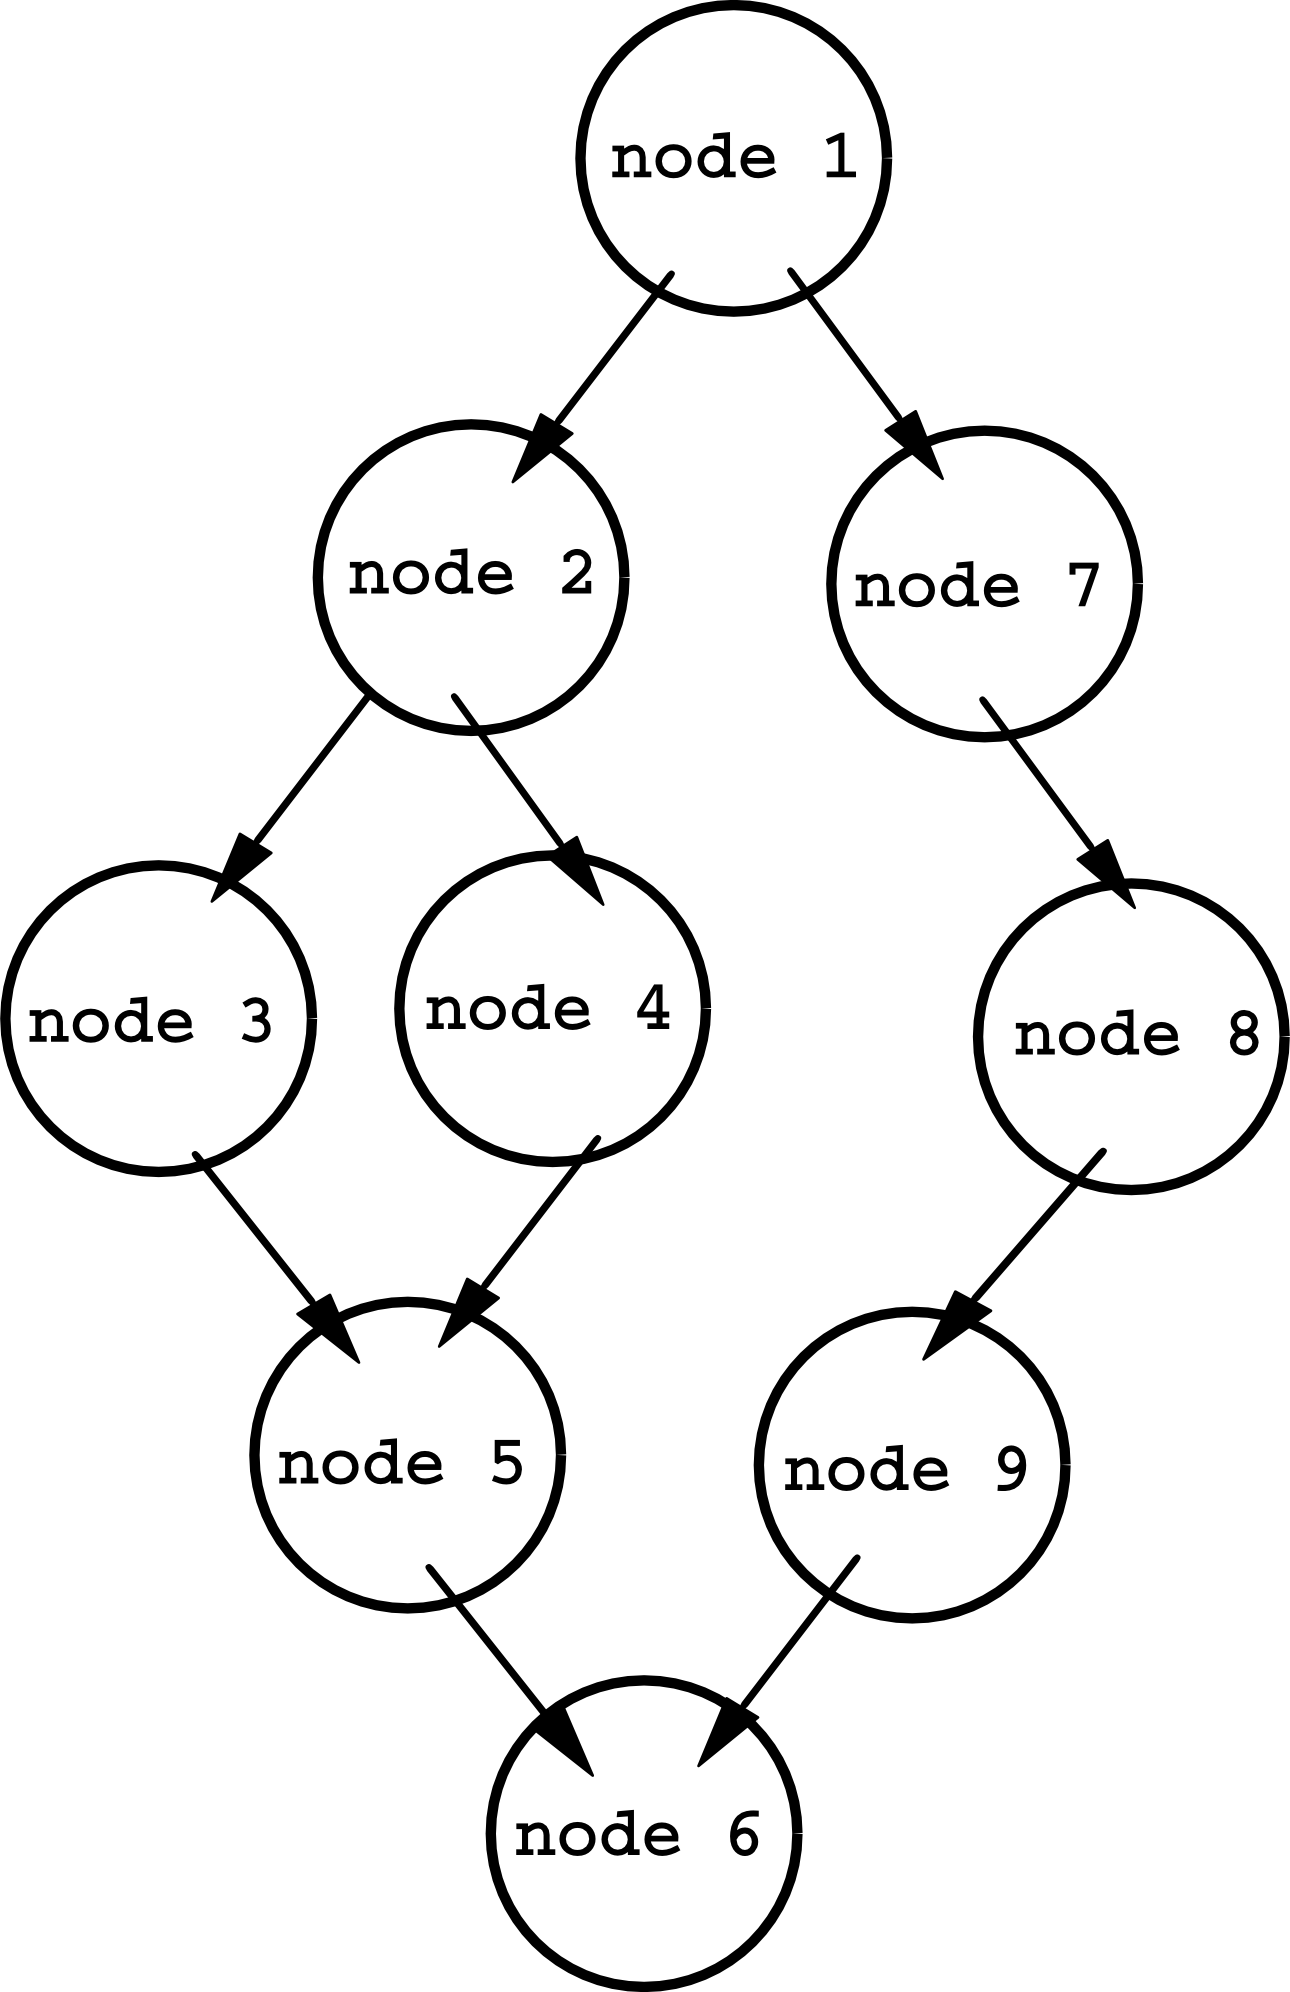
\includegraphics[scale=0.5]{figures/Control_flow_graph}
	\caption{Control Flow Graph.}
	\label{fig:cfg}
\end{figure}

Another example, it tests whether the variables are tainted along the path from Source where the input is provided by the user or untrustworthy and reaches Sink i.e., end of the path without sanitizing the variable. This is called Taint Analysis. It is also called Information Flow Analysis where Information Flow is defined by Dorothy Denning \cite{Denning} as “Information flows from object x to object y, denoted x $\rightarrow$ y , whenever information stored in x is transferred to, object y.” Thereby, the tainted objects are recognised along the flow and depict which are vulnerable. So, overall Static Analysis has great importance in maintaining the quality of code and bug-free before the code went into the production phase. \\ \\


\section{Incremental Static Analysis}

The Static Analysis tools using incremental approach are based on the idea that recalculates only the part of the solution that has been modified by the change in program instead of applying complete original algorithm again. Barbara et. al. introduces ACINCF which is incremental update algorithm for forward data flow analysis and ACINCB for backward data flow analysis. \\ \\

Incremental Static Analysis method was patented by Kalman et al. in the year 2012. The following figure \ref{fig:inc-analysis-fc} illustrates the concept behind it as a flow-chart. \\ \\

\begin{figure}[H]
	\centering
	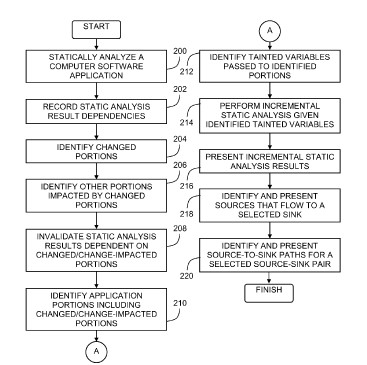
\includegraphics[width=\linewidth]{figures/inc-analysis-fc}
	\caption{Incremental Static Analysis Flow-chart.}
	\label{fig:inc-analysis-fc}
\end{figure}


\section{Layered Static Analysis}

The other advanced approach is Layered Static Analysis patented by Cifuentes et al. in the following year 2013, after Incremental Static Analysis is patented. It is a method which helps in reducing the part of source code having potential bugs. It selects part of Static program analysis in an order of less time required to more for each iteration and slowly eradicating the bug free code. The following figure \ref{fig:lay-analysis-fc} illustrates the concept behind it in more detail as a flow-chart. \\ \\

\begin{figure}[H]
	\centering
	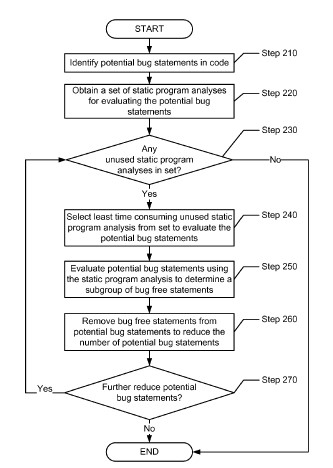
\includegraphics[width=\linewidth]{figures/lay-analysis-fc}
	\caption{Layered Static Analysis Flow-chart.}
	\label{fig:lay-analysis-fc}
\end{figure}


\section{Wireframe}

A wireframe is a methodology of showing a blueprint of a certain product. For example, if we consider to Wireframe a User Interface of an Application. It means to show a blueprint design of how the Application UI look like with different elements like buttons, text boxes etc placed on it and also how they interact and navigate to other User Interfaces. The blueprint design could vary from low fidelity i.e., rough sketches to high fidelity i.e., a more closer look to the desired final UI. There are several tools available in the market to do Wireframe and Balsamiq \cite{B} is one such tool. It is a kind of prototyping the actual product with certain simulation in functionality and visualization of the actual product. The advantage of this is the easiness of finding the mistakes in design earlier and so the cost of fixing them would be less. Here is an example of Website Wireframe is shown in the following figure \ref{fig:wireframe_website} of what one could design using Balsamiq tool and discuss with peers how they feel or to oneself to draw the ideas of what they want to achieve before actually coding to get the web page with the desired UI. \\ \\

\begin{figure}[hbt!]
	\centering
	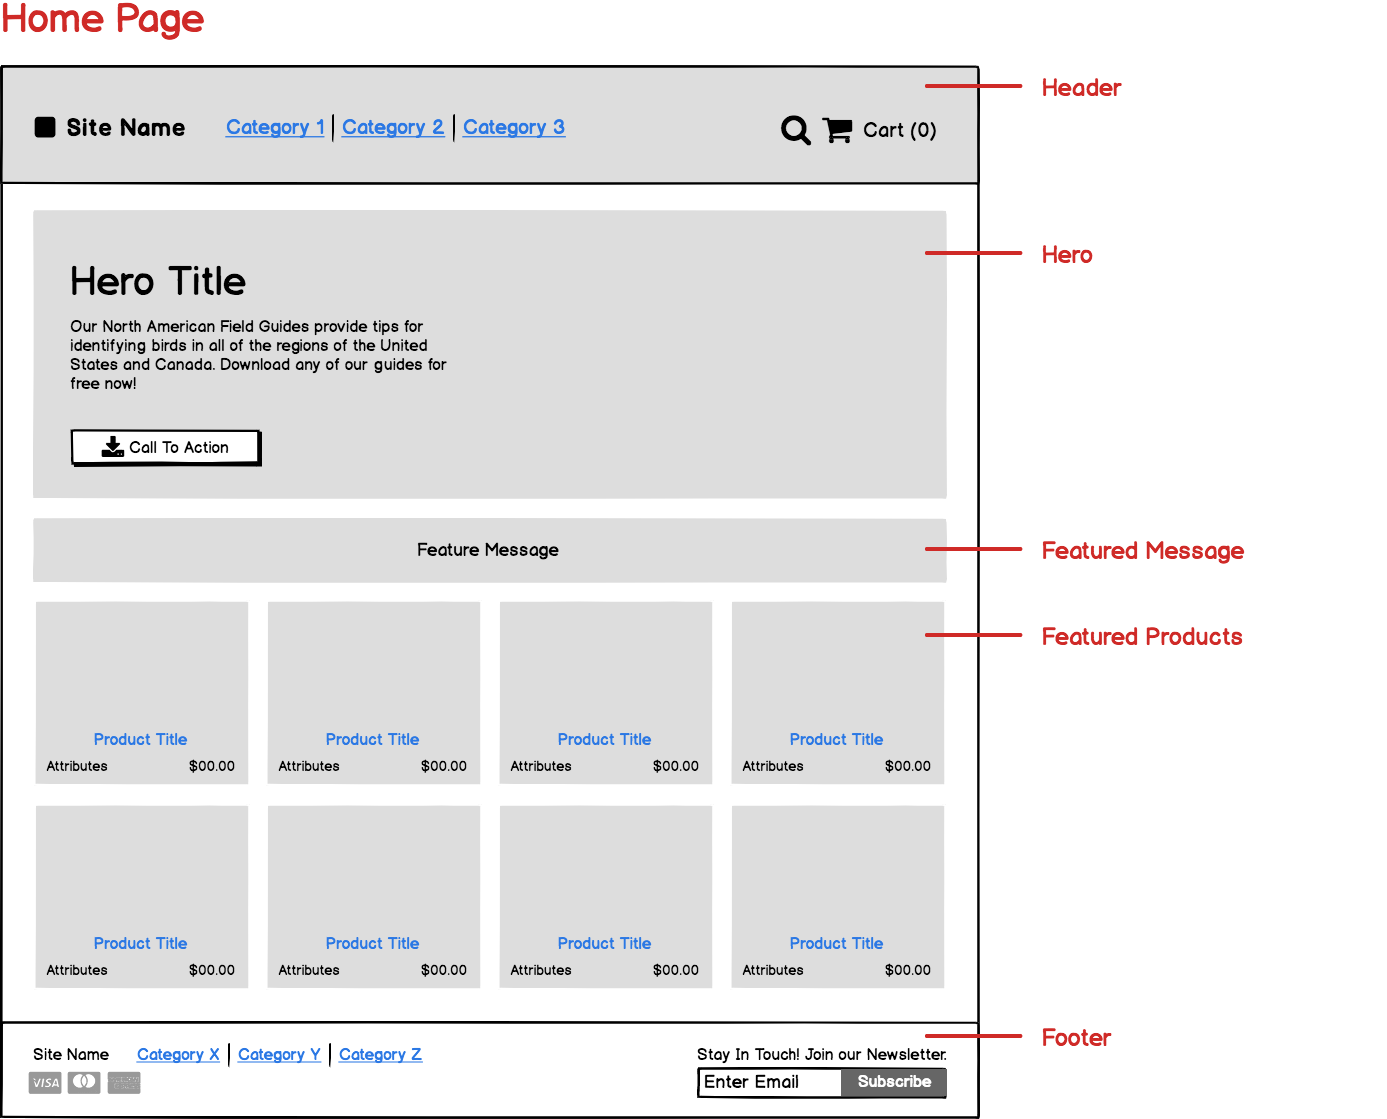
\includegraphics[width=\linewidth]{figures/wireframe_website}
	\caption{Website Wireframe.}
	\label{fig:wireframe_website}
\end{figure}

\section{User Experience Design} 

User Experience ( UX ) Design plays a vital role in the success of a product but often underestimated. In a typical Software Industry, they say reasons to like it might lead to over budget or no time in order to skip it and get right into the development phase. Well, a User Experience Design process is far beyond what we know as User Interface Design or Usability.  User Interface Design is what typically done by Wireframe tool and Usability is a way of testing whether the designed product is usable enough or not. A User Experience ( UX ) Design is a user-centered process which emphasis on the context of the user and his needs than rather focusing solely on interface design. \cite{UX} For example, let us say you designed a navigation application where the user says I want to reach from point A to point B and it displays the route. Now, what if the user wants to mention points as a market name instead of street name and your underlying database consists only street names, that is a bad user experience ( UX ) even though the application is designed with better UI and also Usable. Its Design \cite{UXD} cycle as seen in the figure \ref{fig:ux-design} illustrates an iterative cycle where the requirements are gathered, then a prototype is made on it and evaluated, then again new requirements are gathered based on the evaluation. \\ \\

\begin{figure}[hbt!]
	\centering
	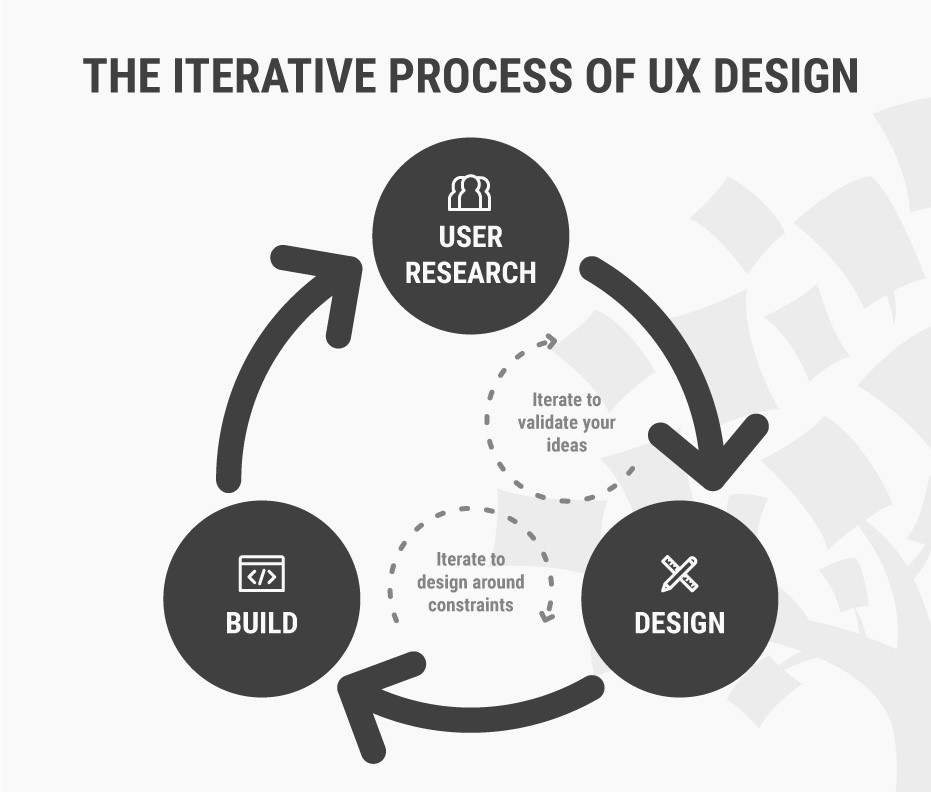
\includegraphics[width=\linewidth]{figures/ux-design}
	\caption{UX-Design.}
	\label{fig:ux-design}
\end{figure}

\let\cleardoublepage\clearpage